%*----------- OBJETIVO GERAL -------------------------------------------------------------
\begin{frame}[c]{Objetivo Geral} 
    \transdissolve[duration=0.5]
   
    \begin{center}
        \Wider{%
        \begin{shaded}
        \begin{center}
            \vspace*{0.4cm}
            \resizebox{!}{1.3cm}{%
                \begin{tabular}{ccc}
                    \textbf{Desenvolver um sistema robótico capaz} \\ 
                    \textbf{de realizar o plantio e monitoramento} \\ 
                    \textbf{de hortaliças}       
                  \end{tabular}
            }%
        \end{center}
        \end{shaded}
        }%
    \end{center}
%*----------- notes
    \note[item]{Notes can help you to remember important information. Turn on the notes option.}
\end{frame}
%-

%*----------- SLIDE -------------------------------------------------------------
\begin{frame}[c]{Projeto similar - FarmBot}
    %\transboxin[duration=1,direction=30]
    \centering

    \includemedia[
      width=0.7\linewidth,
      totalheight=0.39375\linewidth,
      activate=pageopen,
      passcontext, 
      addresource=./Source/movies/introducing-farmbot.mp4,
      flashvars={
      source=./Source/movies/introducing-farmbot.mp4
      &autoPlay=true
      &Loop=false}
      ]{\fbox{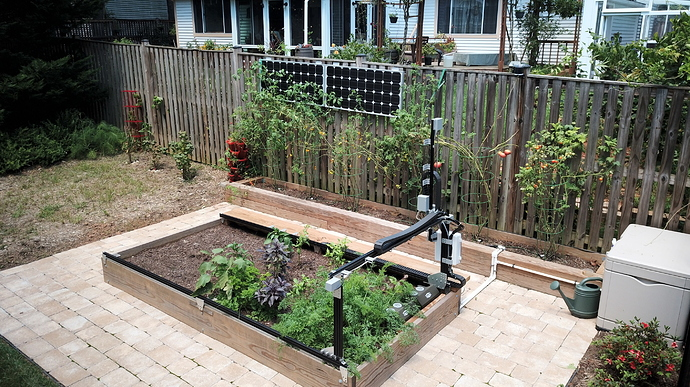
\includegraphics{farmbot.jpeg}}}{VPlayer.swf}

%*----------- notes
    \note[item]{Notes can help you to remember important information. Turn on the notes option.}
\end{frame}

\begin{frame}[t]{Metodologia}
    \begin{figure}
        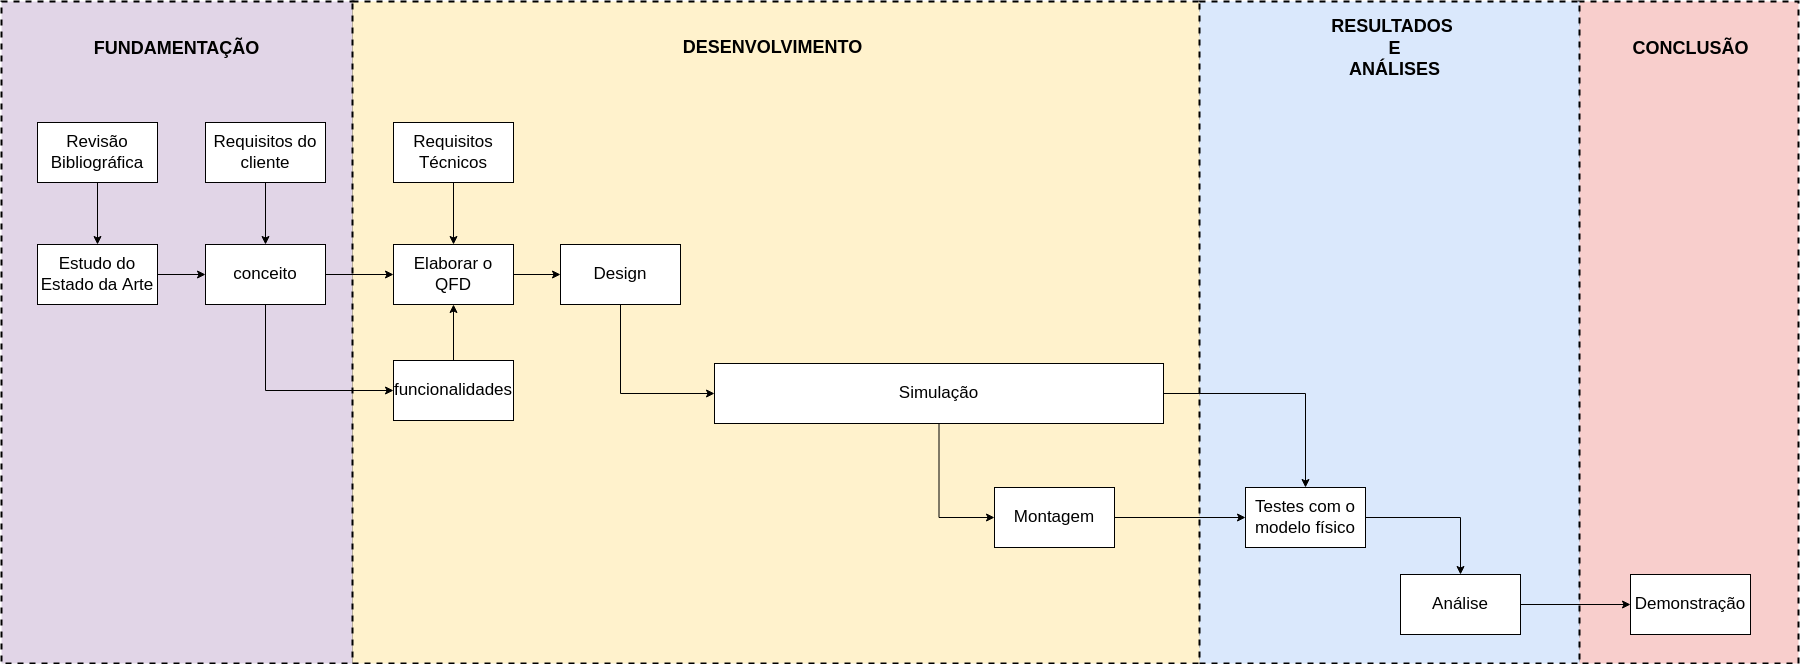
\includegraphics[width=1.005\textwidth]{metodologia.png}
    \end{figure}
%*----------- notes
    \note[item]{Notes can help you to remember important information. Turn on the notes option.}
\end{frame}
%-